\section*{Problems}

\subsection*{Problem statements}

% Remember
\begin{problema}
	\label{prob:f690fbe}
	Write out the terms of each of the following sums:
	\begin{enumerate}
		\item $\displaystyle\sum_{j=0}^{6}X_{j}=$
		\item $\displaystyle\sum_{k=1}^{4}\left( Y_{k}-3 \right)^{2}=$
		\item $\displaystyle\sum_{k=1}^{N}a=$
		\item $\displaystyle\sum_{n=2}^{5}{f_{n}}X_{n}= $
		\item $\displaystyle\sum_{m=0}^{3}\left( X_{m}-a \right)=$
	\end{enumerate}
\end{problema}

% Understand
\begin{problema}
	\label{prob:0b934f5}
	Prove that the sum of the deviations $d_{1},d_{2},...,d_{N}$ of $X_{1},X_{2},...,X_{N}$ around their own mean $\bar{X}$ is equal to zero, and explain why this property justifies describing the arithmetic mean as the "center of gravity" of a data set.
\end{problema}

% Apply
\begin{problema}
	\label{prob:0c7ed43}
	Using the frequency distribution of heights shown in the following table, find the mean height of 100 students at a certain university.
	\begin{figure}[ht]
		\centering
		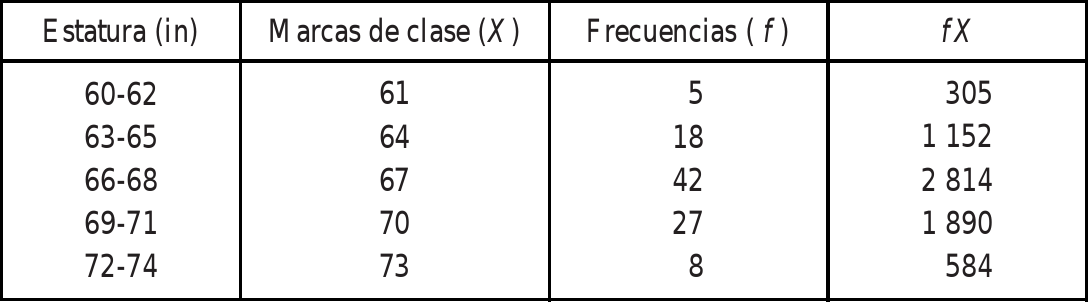
\includegraphics[width=10cm,keepaspectratio=true]{./images/tab0301.png}
		\label{tab:1.2.1-medidas}
	\end{figure}
\end{problema}

% Analyze
\begin{problema}
	\label{prob:08f4f21}
	If the deviations of $N$ numbers $X_{1},..,X_{N}$ with respect to an arbitrary \emph{pivot} $P$ are given by $d_{i}=X_{i}-P, \; i=1,...,N$, prove algebraically that
	\begin{align}
		\bar{X}=P+\dfrac{\sum d_{i}}{N},
	\end{align}
	and verify from this result that the formula is valid regardless of which value of $P$ is chosen.
\end{problema}

% Evaluate
\begin{problema}
	\label{prob:ced3c3b}
	Use the class mark of the central class as the pivot and the coding method based on a change of scale and origin ($u_i = (X_i-P)/c$) to recompute the mean height of the 100 students from Problem \ref{prob:0c7ed43}. Compare the result and the arithmetic effort against the direct computation, and evaluate in which situations (table size, class width, available computing resources) it is preferable to use the coded method instead of the direct method.
\end{problema}

% Create
\begin{problema}
	\label{prob:32476e7}
	An analyst records the response time (in milliseconds) of 60 requests to a web server, grouped in the following frequency table:
	\begin{center}
		\begin{tabular}{cccc}
			\hline
			Interval (ms) & Class mark $X_i$ & Frequency $f_i$ & Cumulative freq. $F_i$ \\
			\hline
			10--19 & 14.5 & 6  & 6 \\
			20--29 & 24.5 & 14 & 20 \\
			30--39 & 34.5 & 22 & 42 \\
			40--49 & 44.5 & 12 & 54 \\
			50--59 & 54.5 & 6  & 60 \\
			\hline
		\end{tabular}
	\end{center}
	Design the complete solution: compute (a) the mean response time $\bar{X}$ using the class marks, and (b) the median response time by linear interpolation in the class containing observation number $N/2=30$.
\end{problema}

\subsection*{Detailed solutions}

% Remember
\begin{solproblema}[prob:f690fbe]
	Expanding each summation term by term according to the indicated indices:
	\begin{enumerate}
		\item $\displaystyle\sum_{j=0}^{6}X_{j} = X_{0} + X_{1} + X_{2} + X_{3} + X_{4} + X_{5} + X_{6}$
		\item $\displaystyle\sum_{k=1}^{4}\left( Y_{k}-3 \right)^{2} = (Y_{1}-3)^{2} + (Y_{2}-3)^{2} + (Y_{3}-3)^{2} + (Y_{4}-3)^{2}$
		\item $\displaystyle\sum_{k=1}^{N}a = \underbrace{a + a + \cdots + a}_{N \text{ times}} = N \cdot a$
		\item $\displaystyle\sum_{n=2}^{5}{f_{n}}X_{n} = f_{2}X_{2} + f_{3}X_{3} + f_{4}X_{4} + f_{5}X_{5}$
		\item $\displaystyle\sum_{m=0}^{3}\left( X_{m}-a \right) = (X_{0}-a) + (X_{1}-a) + (X_{2}-a) + (X_{3}-a)$
	\end{enumerate}
\end{solproblema}

% Understand
\begin{solproblema}[prob:0b934f5]
	Let $d_{i} = X_{i} - \bar{X}$. Summing over all $N$ elements in the data set:
	\begin{align}
		\sum_{i=1}^{N} d_{i} &= \sum_{i=1}^{N} (X_{i} - \bar{X}) = \sum_{i=1}^{N} X_{i} - \sum_{i=1}^{N} \bar{X}.
	\end{align}
	Since $\bar{X}$ is constant with respect to the summation index $i$, $\sum_{i=1}^{N} \bar{X} = N\bar{X}$. Also, by the definition of arithmetic mean, $\sum_{i=1}^{N} X_{i} = N\bar{X}$. Substituting both terms:
	\begin{align}
		\sum_{i=1}^{N} d_{i} = N\bar{X} - N\bar{X} = 0.
	\end{align}
	This property justifies the physical interpretation of the mean as a "center of gravity": just as the balancing point of a system of masses is the point where moments on both sides cancel, the mean is the unique pivot where positive and negative deviations in the data cancel exactly.
\end{solproblema}

% Apply
\begin{solproblema}[prob:0c7ed43]
	From the table, we determine the midpoint or class mark ($X_{i}$) for each height interval (in inches) and multiply it by its frequency $f_{i}$:
	\begin{itemize}
		\item Interval 60--62: $X_{1} = 61$, $f_{1} = 5 \implies f_{1}X_{1} = 305$
		\item Interval 63--65: $X_{2} = 64$, $f_{2} = 18 \implies f_{2}X_{2} = 1152$
		\item Interval 66--68: $X_{3} = 67$, $f_{3} = 42 \implies f_{3}X_{3} = 2814$
		\item Interval 69--71: $X_{4} = 70$, $f_{4} = 27 \implies f_{4}X_{4} = 1890$
		\item Interval 72--74: $X_{5} = 73$, $f_{5} = 8 \implies f_{5}X_{5} = 584$
	\end{itemize}
	Summing the frequencies and products:
	\begin{align}
		N &= \sum f_{i} = 5 + 18 + 42 + 27 + 8 = 100 \\
		\sum f_{i}X_{i} &= 305 + 1152 + 2814 + 1890 + 584 = 6745
	\end{align}
	Therefore, the mean height is:
	\begin{align}
		\bar{X} = \dfrac{6745}{100} = 67.45 \text{ inches.}
	\end{align}
\end{solproblema}

% Analyze
\begin{solproblema}[prob:08f4f21]
	Start from the definition of deviation with respect to the pivot: $d_{i} = X_{i} - P$. Solving for the original variable gives $X_{i} = P + d_{i}$. Summing from $i=1$ to $N$ on both sides of the equality:
	\begin{align}
		\sum_{i=1}^{N} X_{i} &= \sum_{i=1}^{N} (P + d_{i}) = \sum_{i=1}^{N} P + \sum_{i=1}^{N} d_{i} = N \cdot P + \sum_{i=1}^{N} d_{i}.
	\end{align}
	Dividing the whole expression by $N$:
	\begin{align}
		\dfrac{\sum_{i=1}^{N} X_{i}}{N} &= \dfrac{N \cdot P}{N} + \dfrac{\sum_{i=1}^{N} d_{i}}{N} \implies \bar{X} = P + \dfrac{\sum_{i=1}^{N} d_{i}}{N}.
	\end{align}
	This derivation placed no restriction on the value of $P$: it is valid for \emph{any} chosen pivot, whether $P=0$, the mean of another sample, or an arbitrary value, as long as $\sum d_i$ is recomputed with respect to that same $P$. This is exactly what is numerically verified by the invariant result $\bar{X}=9.375$ when using $P=9$ or $P=20$ on the same data set.
\end{solproblema}

% Evaluate
\begin{solproblema}[prob:ced3c3b]
	The class mark of the central interval (66--68) is $P = 67$ inches. Since the classes have constant width $c = 3$ inches, use the coded variable $u_{i} = \dfrac{X_{i} - P}{c}$:
	\begin{itemize}
		\item Cl. 60--62 ($X_{1}=61$): $u_{1} = \frac{61-67}{3} = -2 \implies f_{1}u_{1} = 5(-2) = -10$
		\item Cl. 63--65 ($X_{2}=64$): $u_{2} = \frac{64-67}{3} = -1 \implies f_{2}u_{2} = 18(-1) = -18$
		\item Cl. 66--68 ($X_{3}=67$): $u_{3} = \frac{67-67}{3} = 0 \implies f_{3}u_{3} = 42(0) = 0$
		\item Cl. 69--71 ($X_{4}=70$): $u_{4} = \frac{70-67}{3} = 1 \implies f_{4}u_{4} = 27(1) = 27$
		\item Cl. 72--74 ($X_{5}=73$): $u_{5} = \frac{73-67}{3} = 2 \implies f_{5}u_{5} = 8(2) = 16$
	\end{itemize}
	Summing frequency times code, $\sum f_{i}u_{i} = -10 - 18 + 0 + 27 + 16 = 15$. Applying the shortened mean formula with change of scale and origin:
	\begin{align}
		\bar{X} = P + c\left( \dfrac{\sum f_{i}u_{i}}{N} \right) = 67 + 3\left( \dfrac{15}{100} \right) = 67.45 \text{ inches,}
	\end{align}
	which is identical to the direct result from Problem \ref{prob:0c7ed43}. In terms of arithmetic effort, the coded method replaces products of large numbers (class mark $\times$ frequency, two- and three-digit values) with products of small integers ($-2$ to $2$), reducing the risk of manual calculation error. However, with software or statistical calculators the advantage almost disappears, since both methods are equally fast to execute. Thus, the coded method is mainly useful for manual calculation with large tables or constant class width, not as a systematic substitute in a computerized workflow.
\end{solproblema}

% Create
\begin{solproblema}[prob:32476e7]
	\textbf{(a) Arithmetic mean.} Multiplying each class mark by its frequency:
	\begin{align}
		\sum f_iX_i = 6(14.5)+14(24.5)+22(34.5)+12(44.5)+6(54.5) = 87+343+759+534+327 = 2050.
	\end{align}
	With $N=60$:
	\begin{align}
		\bar{X} = \dfrac{2050}{60} \approx 34.17 \text{ ms.}
	\end{align}
	\textbf{(b) Median by interpolation.} We identify the class containing observation $N/2=30$: the cumulative frequency reaches $F=20$ at the end of class 20--29 and $F=42$ at the end of class 30--39, so the median class is 30--39, with lower real limit $L_m=29.5$, previous cumulative frequency $F_{m-1}=20$, class frequency $f_m=22$, and width $c=10$:
	\begin{align}
		Med = L_m + \left( \dfrac{N/2 - F_{m-1}}{f_m} \right)c = 29.5 + \left( \dfrac{30-20}{22} \right)(10) = 29.5 + 4.55 = 34.05 \text{ ms.}
	\end{align}
	The mean ($34.17$ ms) and median ($34.05$ ms) are very close, which is consistent with a response-time distribution that is reasonably symmetric around the central class.
\end{solproblema}
